% -----------------------------------------------
% Template for ICMC 2005
%     icmc.sty -> style file
% By Eloi Batlle (eloi@iua.upf.es), changes for 
% ICMC 2005 by Bram de Jong 
% Adapted for the ICMC 2008 by Maarten van Walstijn
% -----------------------------------------------

\documentclass{article}
\usepackage{icmc,amsmath}
\usepackage{graphicx}
\usepackage{hyperref}
\usepackage{url}
\usepackage{color}
\definecolor{black}{rgb}{0,0,0}
\hypersetup{colorlinks,urlcolor=black,linkcolor=black,citecolor=black}  
%reduces the space between the items in the itemize-environment 
\newenvironment{packed_enumerate}{
\begin{enumerate}
  \setlength{\itemsep}{1pt}
  \setlength{\parskip}{0pt}
  \setlength{\parsep}{0pt}
}{\end{enumerate}}
\newenvironment{packed_item}{
\begin{itemize}
  \setlength{\itemsep}{1pt}
  \setlength{\parskip}{0pt}
  \setlength{\parsep}{0pt}
}{\end{itemize}}

% Title.
% ------
% CHANGED: New title -- this paper is really about what we are doing with parameters
\title{The Development of a Multifaceted Parameter Model in Jamoma}

% Single address
% To use with only one author or several with the same address
% ---------------
%\oneauthor
%  {Author} {School \\ Department}

% Two addresses
% --------------
%\twoauthors
%  {First author} {School \\ Department}
%  {Second author} {Company \\ Address}

% Three addresses
% --------------
\threeauthors
  {First author} {School \\ Department}
  {Second author} {Company \\ Address}
  {Third author} {Company \\ Address}

\begin{document}
%
\maketitle
%
\sloppy
%%%%%%%%%%%%%%%%%%%%%%%%%%%%%%%%%%%%%%%%%%%%%%%%%%%%%%%%%%%%%%%%%%%%%%%%%%%%%%%
%%%%%%%%%%%%%%%%%%%%%%%%%%%%%%%%%%%%%%%%%%%%%%%%%%%%%%%%%%%%%%%%%%%%%%%%%%%%%%%
%%%%%%%%%%%%%%%%%%%%%%%%%%%%%%%%%%%%%%%%%%%%%%%%%%%%%%%%%%%%%%%%%%%%%%%%%%%%%%%
\begin{abstract}
%The abstract should be placed at the top left column and should contain
%about 150-200 words.

A prototype implementation in Jamoma is presented and discussed.


\end{abstract}


%%%%%%%%%%%%%%%%%%%%%%%%%%%%%%%%%%%%%%%%%%%%%%%%%%%%%%%%%%%%%%%%%%%%%%%%%%%%%%%
%%%%%%%%%%%%%%%%%%%%%%%%%%%%%%%%%%%%%%%%%%%%%%%%%%%%%%%%%%%%%%%%%%%%%%%%%%%%%%%
%%%%%%%%%%%%%%%%%%%%%%%%%%%%%%%%%%%%%%%%%%%%%%%%%%%%%%%%%%%%%%%%%%%%%%%%
\section{Introduction} % (fold)
\label{sec:introduction}

% CHANGED [ARJ] This looked more like an introduction than an abstract. Parts of it could probably be moved to the introduction instead?
% TODO [ARJ] It is good to have a more conceptual start, but right now it feels a bit too conceptual. "materials" and "plasticity" should probably be outlined some more.
Fundamental to the development of musical or artistic material is the ability to transform raw materials.  This ability implies the facility to master many facets of the material, and to manipulate it with plasticity.  Computer music environments typically provide points of control to manipulate material by providing parameters with controllable values. However, we find that this capability to control the values of parameters is inadequate for many of our artistic endeavors, and does not reflect the analogous tools and methods of artists working with physical materials. For this reason we have started to explore alternative ways of working with dynamic structures.

A possible partial solution is to treat a parameter not as a single-value representing entity, but to treat a parameter as a multi-dimensional tool or object.  Thus the parameter, as a tool or object, has many facets itself in addition to the value it renders.  These many \emph{properties} of the parameter define its behavior. This paper presents a prototype of these ideas, implemented in Jamoma, a modular framework for Max/MSP \cite{Place:2006}. In addition to defining behaviors, the behaviors are themselves interdependent upon each other requiring a flexible and dynamically bound code base for the implementation.

% TODO: Main question:
% We've done quite a lot of work, and here is what we've done.
% Why did we do this?
% What's the point?

% How do we transition from this stuff to the more concrete?
% Conceptual idea: 
% - materials
% - plasticity
% 
% (model and work with..., living entity)

% section introduction (end)



%%%%%%%%%%%%%%%%%%%%%%%%%%%%%%%%%%%%%%%%%%%%%%%%%%%%%%%%%%%%%%%%%%%%%%%%%%%%%%%
%%%%%%%%%%%%%%%%%%%%%%%%%%%%%%%%%%%%%%%%%%%%%%%%%%%%%%%%%%%%%%%%%%%%%%%%%%%%%%%
%%%%%%%%%%%%%%%%%%%%%%%%%%%%%%%%%%%%%%%%%%%%%%%%%%%%%%%%%%%%%%%%%%%%%%%%%%%%%%%
\section{Model-View-Controller} %(fold)
% TODO [ARJ] Probably better to link to a publication rather than Wikipedia. I took the first I found on google scholar, but there might be a more relevant publication. [NP] is this definition so important? Instead I would just include a screenshot of a small Jamoma patch and then briefly explain the Jamoma concept by refering to them. 

Jamoma is a Model-View-Controller (MVC) framework that supplies a modular structure for the Max/MSP environment. ``MVC programming is the application of [a] three-way factoring, whereby objects of different classes take over the operations related to the application domain (the model), the display of the application's state (the view), and the user interaction with the model and the view (the controller).'' \cite{Krasner:1988}  In Jamoma, the model is represented as a Max patcher or external object called the \emph{algorithm}.  The user interface, embedded in a patcher or bpatcher is the view.  The controller is composed of a collection of interacting and dynamically-bound objects, which we refer to as the \emph{Jamoma Core}.

% TODO: Tie the above paragraph to the below paragraph.  If the paragraph above is split up, it could be that each of the M, the V, and C are given their own paragraphs, and the paragraph below is in the discussion of the controller.  This allows us to still provide our definitions up front, while not boringly saying "here are a bunch of definitions".

The messaging model in Jamoma addresses modules using \emph{parameters} (i.e. nodes with state) and \emph{messages} (i.e. nodes which are stateless). For the duration of this paper we will often refer only to parameters, but the concepts generally apply to both parameters and messages.

% (end)


%%%%%%%%%%%%%%%%%%%%%%%%%%%%%%%%%%%%%%%%%%%%%%%%%%%%%%%%%%%%%%%%%%%%%%%%%%%%%%%
%%%%%%%%%%%%%%%%%%%%%%%%%%%%%%%%%%%%%%%%%%%%%%%%%%%%%%%%%%%%%%%%%%%%%%%%%%%%%%%
%%%%%%%%%%%%%%%%%%%%%%%%%%%%%%%%%%%%%%%%%%%%%%%%%%%%%%%%%%%%%%%%%%%%%%%%%%%%%%%
\section{Dynamic Binding} % (fold)
\label{sec:dynamic_binding}

% Changed: Changed "audiomusical" to using the term "time-based art". See e.g. http://www.pica.org/tba/ for examples of the use of this term. [TL]
For our purposes we will assume the \emph{materials} we are working with to be media related to time-based art, such as real-time processing of audio, video, midi or other kinds of data as part of a performance. The plasticity we refer to means we want to easily shape and mold our materials into a final sonic or visual output.

% TODO: Move this type of stuff up to section 1 so we are more clear about stating the problem.
Current practice for many users of computer music software is predicated on static relationships and the use of static presets. This is certainly true for many Digital Audio Workstations (DAWs) whose overall structure is fixed. It is, however, also true of open-ended systems, such as PureData or Max/MSP. In a graphical environment, the relationships between objects and their interconnections form the algorithm that determines a tools behavior. Within this algorithm there is typically some freedom to modify its behavior by e.g. changing coefficients. However, the objects and connections generally do not change on-the-fly as a performance is executed.

Many of these systems, Max/MSP in particular, have provisions for breaking out of sets of static relationships through scripting. For the vast majority of users, however, mastering this task is onerous at best. By keeping these relationships fixed, the expressivity available to the user is inherently limited.

% TODO: How to cite the thing in the footnote below? [TAP]
% NOTE: I've done a lot of searching for something more 'academic' on dynamic binding, but was not able to turn up anything good. [TAP]
Jamoma aims to address this through the use of \emph{dynamic binding}. One prevalent example of dynamic binding is the Objective-C language. Static binding ``constraints are limiting because they force issues to be decided from information found in the programmer’s source code, rather than from information obtained from the user as the program runs.''\footnote{\url{http://developer.apple.com/documentation/Cocoa/Conceptual/OOP_ObjC/Articles/chapter_5_section_6.html}}

Dynamic binding in Jamoma takes place on several levels.  At the highest level, a module's parameters are bound to its hub dynamically to form the Controller layer of the MVC paradigm.  Then dynamic binding takes place inside of the parameters as its properties are changed.

% CHANGED: I don't think we really need this. The focus of this paper is really on the parameter itself, not on the module as a whole...  [TAP]
%%%%%%%%%%%%%%%%%%%%%%%%%%%%%%%%%%%%%%%%%%%%%%%%%%%%%%%%%%%%%%%%%%%%%%%%%%%%%%%
%\subsection{The Subscription System}
%
%Parameters are bound dynamically to a module.  When a Max patcher loads a module, that module creates a \emph{hub} object which acts as the controller for everything in the module. As parameters are created they subscribe to the hub to form a bi-directional connection for exchanging data.  The existence of parameters may even change over the course of time, and in response to changes in other parameters.
%
%\subsection{Parameter Components}

% section dynamic_binding (end)

\begin{figure}
\centerline{\framebox{
	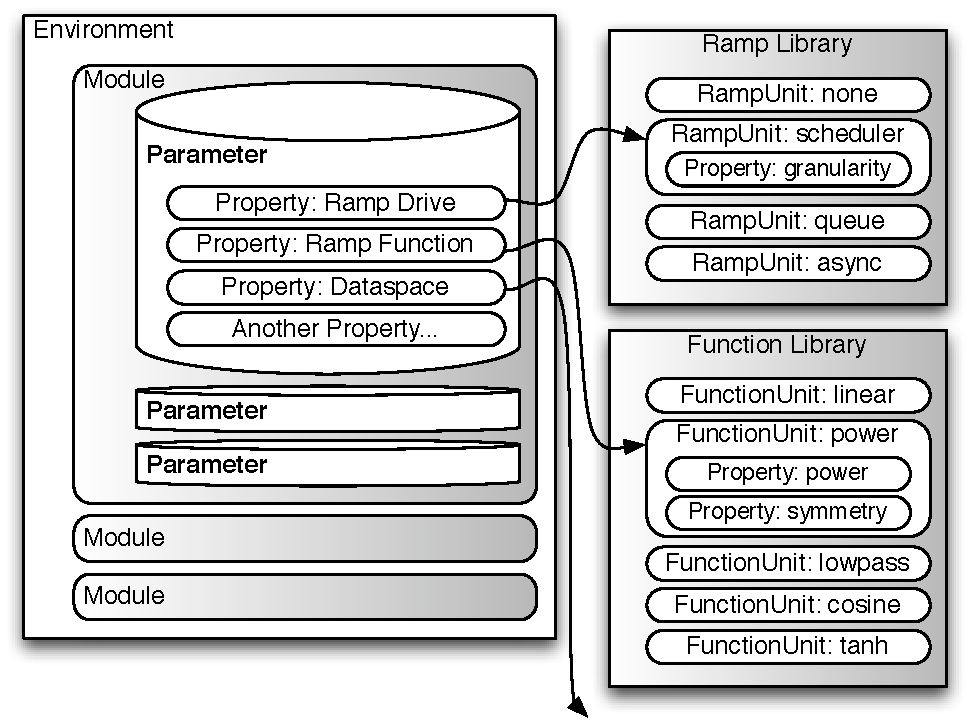
\includegraphics[width=\columnwidth]{figure-structure}}}
\caption{An OSC address tree, with some nodes as classes}
\label{fig:structure}
\end{figure}


%%%%%%%%%%%%%%%%%%%%%%%%%%%%%%%%%%%%%%%%%%%%%%%%%%%%%%%%%%%%%%%%%%%%%%%%%%%%%%%
%%%%%%%%%%%%%%%%%%%%%%%%%%%%%%%%%%%%%%%%%%%%%%%%%%%%%%%%%%%%%%%%%%%%%%%%%%%%%%%
%%%%%%%%%%%%%%%%%%%%%%%%%%%%%%%%%%%%%%%%%%%%%%%%%%%%%%%%%%%%%%%%%%%%%%%%%%%%%%%
\section{The Parameter} %(fold)
\label{sec:the_parameter}

% TODO: Add a figure showing the structure of the parameter, methods, properties, etc. -- put it in more conceptual section
% TODO: This paragraph belongs in the conceptual section
The parameter is the primary interface for a user manipulating the state of a module. In most systems, the parameter has a single task: to set a variable or coefficient. While it is straightforward to understand such a simple 1-dimensional control, it does not offer the degree of nuance that, say, a sculptor has when working with clay.

In Jamoma, the parameter is made multi-dimensional through the use of \emph{properties} and \emph{methods} in addition to maintaining the state of a value \cite{Place:2008}. These properties define the behavior for parameters by setting a value range, repetition filtering, the type of units used to express values, and how automation is applied. The following is list of available properties and methods for any given parameter.

% TODO: Here begins specific Jamoma stuff that is a prototype

Following is a list of the properties and methods of a parameter.
\begin{center} 
{\footnotesize
\begin{tabular}{ll}
	\texttt{:/value} & The value of the parameter. \\
	\texttt{:/value/stepsize} & The size of the step taken by the inc and dec messages. \\
	\texttt{:/value/inc} & Increase the value of the parameter by the stepsize. \\
	\texttt{:/value/dec} & Decrease the value of the parameter by the stepsize. \\
	\texttt{:/value/default} & The initial value of a parameter when the module is first created. \\
	\texttt{:/type} & The type of data represented by the parameter. \\
	\texttt{:/priority} & The value of the parameter. \\
	\texttt{:/ui/freeze} & The value of the parameter. \\
	\texttt{:/ui/refresh} & The value of the parameter. \\
	\texttt{:/ramp/drive} & The value of the parameter. \\
	\texttt{:/ramp/function} & The value of the parameter. \\
	\texttt{:/repetitions} & The value of the parameter. \\
	\texttt{:/range/bounds} & The value of the parameter. \\
	\texttt{:/range/clip} & The value of the parameter. \\
	\texttt{:/description} & The value of the parameter. \\
	\texttt{:/node/type} & The value of the parameter. \\
	\texttt{:/node/name} & The value of the parameter. \\
	\texttt{:/dataspace} & The value of the parameter. \\
	\texttt{:/dataspace/unit/active} & The value of the parameter. \\
	\texttt{:/dataspace/unit/native} & The value of the parameter. \\
\end{tabular} } 
\end{center}  

A parameter's behavior is ultimately determined by a compendium of these properties. Some properties are simple values, such as the \texttt{:/repetitions} property. Other properties may be a dynamic object which itself possesses a number of properties.  Such properties include the \texttt{:/ramp/drive}, \texttt{:/ramp/function}, and various \texttt{:/dataspace} properties.

%%%%%%%%%%%%%%%%%%%%%%%%%%%%%%%%%%%%%%%%%%%%%%%%%%%%%%%%%%%%%%%%%%%%%%%%%%%%%%%
\subsection{Implementation} % (fold)

% subsection properties_and_methods (end)

% TODO: Tie this subsection into the previous paragraph better [TAP]

The parameter is implemented as a Max external called \emph{jcom.parameter}. Within jcom.parameter, the ramp and dataspace properties are implemented internally as dynamically bound objects using the TTBlue framework\footnote{\url{http://www.electrotap.com/ttblue/}}.  The TTBlue framework is a C++ library that implements a dynamic messaging layer rather than using statically-linked C/C++ function calls \cite{Place:2008ttblue}.  

By using dynamically linked components inside of the parameter, it is possible to switch between many different options for a give parameter property, while each option may implement an entirely different set of methods.  This will be demonstrated in upcoming sections.

% section implementation (end)



%%%%%%%%%%%%%%%%%%%%%%
% TODO: This may have no place here, who knows...  We cut it from the NIME paper [TAP]  It depends on how detailed we want to be with all of the various properties...  It doesn't really pertain to the topic of the dynamic components in a parameter.
%\subsection{Controlling the User Interface} % (fold)
%\label{sub:controlling_the_user_interface}
%
%In certain applications the CPU overhead of continuously updating the graphical user interface whenever parameter or message values change might become a burden, competing for CPU with e.g. video processing algorithms. If the user does not need continuous visual feedback on updated values of parameters or messages, the GUI for the parameter or message can be frozen, freeing up the processor and GPU for tasks considered more important:
%
%\texttt{:/ui/freeze}
%
%\texttt{:/ui/freeze/get}
%
%A parameter or message that has its GUI frozen can be forced to update and refresh the displayed value once by means of the message:
%
%\texttt{:/ui/refresh}

% subsection controlling_the_user_interface (end)



%%%%%%%%%%%%%%%%%%%%%%%%%%%%%%%%%%%%%%%%%%%%%%%%%%%%%%%%%%%%%%%%%%%%%%%%%%%%%%%
%%%%%%%%%%%%%%%%%%%%%%%%%%%%%%%%%%%%%%%%%%%%%%%%%%%%%%%%%%%%%%%%%%%%%%%%%%%%%%%
%%%%%%%%%%%%%%%%%%%%%%%%%%%%%%%%%%%%%%%%%%%%%%%%%%%%%%%%%%%%%%%%%%%%%%%%%%%%%%%
\section{The Jamoma Libraries} % (fold)
\label{sec:the_jamoma_libraries}

The functionality we refer to within a parameter is implemented in a shared library. Within the shared library the different functionalities are grouped in a series of ``Libs''.  These libraries provide the key functionalities for developing multidimensional tools.  To date, the libs are composed of:
\begin{itemize}
	\item FunctionLib: a library of FunctionUnits which map an input value to an output value
	\item RampLib: a library of driving mechanisms (RampUnits) which use the FunctionLib to automate value transformations over time.
	\item DataspaceLib: a library by which a parameter or message can be given a class that describes the type of data it represents.  Values may then be set by any of a number of DataspaceUnits to allow control of a parameter in any of a number of ways.
\end{itemize}



Why do we need to work with Functions and Ramps and Dataspaces:
- we have ramps everywhere -> dynamic (reconfigurable) non-static
    - different functions
    - much more flexible than pattr
    

Things in Common among the 3:
So that we have a library
- shared so that everywhere we need it we can access it
- easily extendable
- queryable



%%%%%%%%%%%%%%%%%%%%%%%%%%%%%%%%%%%%%%%%%%%%%%%%%%%%%%%%%%%%%%%%%%%%%%%%%%%%%%%
%%%%%%%%%%%%%%%%%%%%%%%%%%%%%%%%%%%%%%%%%%%%%%%%%%%%%%%%%%%%%%%%%%%%%%%%%%%%%%%
%%%%%%%%%%%%%%%%%%%%%%%%%%%%%%%%%%%%%%%%%%%%%%%%%%%%%%%%%%%%%%%%%%%%%%%%%%%%%%%
\subsection{The Ramp Library} % (fold)
\label{sec:ramplib}

% TODO: gear this more towards artistic, and less toward technical implementation. Try to explain the motivation for the design decisions we've made.

Jamoma offers vastly extended possibilities in how ramping can be done as compared to Max. In Jamoma the process of ramping is made up from the combination of two components: A driving mechanism cause calculations of new values at desired intervals during the ramp, while a set of functions offers a set of curves for the ramping. Both components are implemented as C++ APIs, and can easily be extended with new ramp or function \emph{units}, expanding the range of possible ramping modes. %TODO: Is this important for the ICMC audience that the Ramplib API is made with C++ and that it be can easily extended? [NP]

The Jamoma RampLib API provides a means by which to create and use \emph{ramp units} in Jamoma.  A ramp unit is a self-contained algorithm that can slide from an existing value to a new value over a specified amount of time according to different timing mechanisms. Each ramp unit is implemented in the form of two C++ files: a source file and a header file that provides an interface for the source file. Currently four such ramp units are implemented:

\begin{itemize}
	\item \emph{none} - jumps immediately to the new value. Typically used for values where ramping do not make sense.
	\item \emph{scheduler} - use the Max internal clock to generate new values at fixed time intervals.
	\item \emph{queue} - ramping using the Max queue, updating values whenever the processor has free capacity to do so.
	\item \emph{async} - only calculate new values when requested to do so. This might be used in video processing modules to calculate fresh values immediately before processing the next video image or matrix.
\end{itemize}

When a new ramp is started, the ramp unit internally use a normalized ramping value, increasing linearly from $0.0$ to $1.0$ over the duration of the ramp. Whenever the ramp unit is to provide a new value, it updates the normalized ramping value, and pass it to a Function Unit as described in Section~\ref{sec:function_lib}. The normalized value returned is then scaled to the range defined by the start and end values for the ramp, and passed on to the module.


% subsection ramplib (end)


%%%%%%%%%%%%%%%%%%%%%%%%%%%%%%%%%%%%%%%%%%%%%%%%%%%%%%%%%%%%%%%%%%%%%%%%%%%%%%%
\subsection{The Function Library} % (fold)
\label{sec:functionlib}
The Jamoma FunctionLib API provides normalized mappings of values $x \in [0,1]$ to $y \in [0,1]$ according to functions $y = f(x)$. The FunctionLib can easily be expanded by introducing new functions in the form of two C++ files: a source file and a header file that provides an interface for the source file.

Currently five functions are implemented: 

\begin{itemize}
	\item Linear: $y = x$.
	\item Cosine: $y = - \frac{1}{2} \cdot cos(x \cdot \pi ) + \frac{1}{2} $.
	\item Lowpass series: $y[n] = y[n-1] \cdot k + x[n] \cdot (1-k)$, \\ where $k$ is a feedback coefficient.
	\item Power function: $ y = x^{k} $, parameter $k$ can be set.
	\item Hyperbolic tangent: $ y = c \cdot (\tanh(a\cdot(x-b)) - d) $, \\ where coefficients $a$, $b$, $c$, $d$ depends on the width and offset of the curve.
\end{itemize}



\begin{table}
\begin{center}
\begin{tabular}{|l|l|l|l|l|l|}
\hline
          & Cosine & Linear & Lowpass & Power & Tanh \\
\hline
Scheduler &        &   x    &         &       & \\
\hline
Queue	  &        &        &         &       & \\
\hline
None	  &        &        &         &       & \\
\hline
Async	  &        &        &         &       & \\
\hline
\end{tabular}
\end{center}
\caption{The possible ramping configurations in Jamoma}
\label{tab:ramp_possibilities} %FIXME: this table has no reference to the text
\end{table}

% section functionlib (end)


%%%%%%%%%%%%%%%%%%%%%%%%%%%%%%%%%%%%%%%%%%%%%%%%%%%%%%%%%%%%%%%%%%%%%%%%%%%%%%%
\subsection{The Dataspace Library} %(fold)
\label{sec:dataspacelib}
The DataspaceLib is important because...
using different unit types and moving toward more perceptual/semantic representations instead of being chained to technical terms.



It will be good for us to try and explain all the interactions here ;-) 
\begin{packed_item}
	\item AngleDataspace
	\item NoneDataspace
	\item ColorDataspace
	\item PitchDataspace
	\item PositionDataspace
	\item DistanceDataspace
    \item TemperatureDataspace
    \item GainDataspace
	\item TimeDataspace
\end{packed_item}
	


%%%%%%%%%%%%%%%%%%%%%%%%%%%%%%%%%%%%%%%%%%%%%%%%%%%%%%%%%%%%%%%%%%%%%%%%%%%%%%%
\subsection{TemperatureDataspace}\label{subsec:temperature_dataspace}

La de da...right now 1ºC in Montreal %TODO: not necessary, or should go to the Dataspace subsection [NP]



\section{Interdependencies}\label{sec:interdependencies}

This paper discusses the structure and development of the interrelated libraries that are used to implement this system.

% subsection dataspacelib (end)
% section the_jamoma_libraries (end)


%%%%%%%%%%%%%%%%%%%%%%%%%%%%%%%%%%%%%%%%%%%%%%%%%%%%%%%%%%%%%%%%%%%%%%%%%%%%%%%
%%%%%%%%%%%%%%%%%%%%%%%%%%%%%%%%%%%%%%%%%%%%%%%%%%%%%%%%%%%%%%%%%%%%%%%%%%%%%%%
%%%%%%%%%%%%%%%%%%%%%%%%%%%%%%%%%%%%%%%%%%%%%%%%%%%%%%%%%%%%%%%%%%%%%%%%%%%%%%%
\section{Discussion and further work} % (fold)
\label{sec:discussion_and_further_work}

The problem: 
It has been too static
    - too difficult to create dynamic setups
    - for example, dynamic setups in Max using scripting: ick!

Trying to create something that is more flexible, but also easier to work with at the same time.

Splitting up and identify the way we handle structures in Max and put them together.  It has been very static and preset-based.

As we've been working on this for along, we hit a wall and needed to move forward, and did so by creating these libs to extend Max.  

No one wants to have to manually do all of the house-keeping to get this functionality, so we've made it largely encapsulated behind the scenes.


\cite{Momeni:2003}



4 ramp units times 5 function units = 20 ramping modes

ramp units can be used for other scheduled processes as well

Possibility of expanding ramp units as low frequency oscillators

function units can be used elsewhere, e.g. for mapping

Audio rate ramp unit.

DataspaceLib

Querying - we propose a different system to the Lemur OSC2 draft

Ramp Lib and Function Lib can be used outside the context of jcom.parameter and jcom.value: jcom.map and jcom.ramp


Plans to extend the FunctionLib by introducing exponential functions are under discussion. %CHANGED: move this from the FunctionLib to Future Work [NP] 


* ramping with our own scheduler to take the burden off of the Max scheduler.



% section discussion_and_further_work (end)


%\begin{thebibliography}{citations}
%
%\bibitem{Author:00} Author, E.
%''The title of the conference paper'',
%{\it Proceedings of the International Computer Music Conference}, Miami, USA, 2004.
%
%\bibitem{Someone:02} Someone, A.
%{\it  Title of the book}.
%Publisher, Belfast, 2007.
%
%\end{thebibliography}

% Bibliography (fold)
%
% The following two commands are all you need in the initial runs of your .tex file to
% produce the bibliography for the citations in your paper.
% CHANGED: I remove the small again for the bibliography, since this isn't used in the template.
%\begin{small}
\bibliographystyle{abbrv}
\bibliography{jamoma-icmc2008}  % the name of the Bibliography in this case
%\end{small}
% You must have a proper ".bib" file
%  and remember to run:
% latex bibtex latex latex
% to resolve all references
%
% Bibliography (end)



\end{document}
